\textbf{Contributions}

The material in this chapter expands on work presented in

~\autocite{cassellaExactChiralAmorphous2022} Cassella, G., D'Ornellas, P., Hodson, T., Natori, W. M., \& Knolle, J. (2022). An exact chiral amorphous spin liquid. \emph{arXiv preprint arXiv:2208.08246.}

the code is available at~\autocite{hodsonKoalaKitaevAmorphous2022}.

This was a joint project of Gino, Peru and myself with advice and guidance from Willian and Johannes. The project grew out of an interest the three of us had in studying amorphous systems, coupled with Johannes' expertise on the Kitaev model. The idea to use voronoi partitions came from~\autocite{marsalTopologicalWeaireThorpe2020} and Gino did the implementation of this. The idea and implementation of the edge colouring using SAT solvers, the mapping from flux sector to bond sector using A* search were both entirely my work. Peru found the ground state and implemented the local markers. Gino and I did much of the rest of the programming for Koala while pair programming and 'whiteboard'ing, this included the phase diagram, edge mode and finite temperature analyses as well as the derivation of the projector in the amorphous case.

\hypertarget{amk-Model}{%
\section{The Model}\label{amk-Model}}

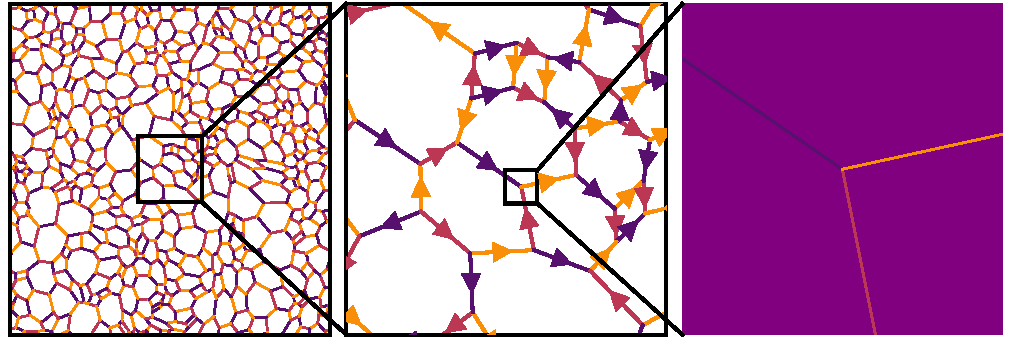
\includegraphics[width=1\textwidth,height=\textheight]{figure_code/amk_chapter/intro/amk_zoom/amk_zoom} 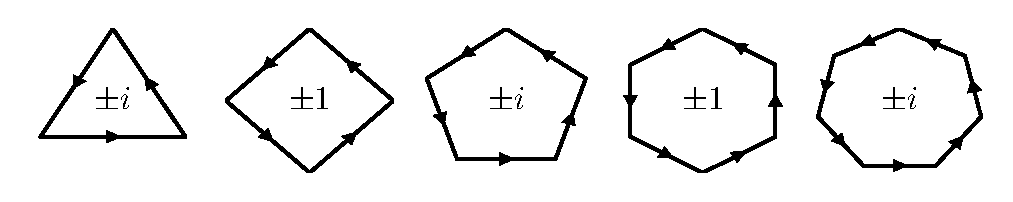
\includegraphics[width=0.86\textwidth,height=\textheight]{figure_code/amk_chapter/intro/regular_plaquettes/regular_plaquettes}

\hypertarget{amorphous-systems}{%
\subsection{Amorphous Systems}\label{amorphous-systems}}

\textbf{Insert discussion of why a generalisation to the amorphous case is interesting}

This chapter details the physics of the Kitaev model on amorphous lattices.

It starts by expanding on the physics of the Kitaev model. It will look at the gauge symmetries of the model as well as its solution via a transformation to a Majorana hamiltonian. This discussion shows that, for the the model to be solvable, it needs only be defined on a trivalent, tri-edge-colourable lattice~\autocite{Nussinov2009}.

The methods section discusses how to generate such lattices and colour them. It also explain how to map back and forth between configurations of the gauge field and configurations of the gauge invariant quantities.

The results section begins by looking at the zero temperature physics. It presents numerical evidence that the ground state of the Kitaev model is given by a simple rule depending only on the number of sides of each plaquette. It assesses the gapless, Abelian and non-Abelian, phases that are present, characterising them by the presence of a gap and using local Chern markers. Next it looks at spontaneous chiral symmetry breaking and topological edge states. It also compares the zero temperature phase diagram to that of the Kitaev Honeycomb Model. Finally, we introduce flux disorder and demonstrate that there is a phase transition to a thermal metal state.

The discussion considers possible physical realisations of this model and the motivations for doing so. It also discusses how a well known quantum error correcting code defined on the Kitaev Honeycomb model could be generalised to the amorphous case.

Lieb's theorem is only valid for bipartite, translation invariant lattices like the honeycomb. Luckily, extensive numerical simulations have shown that the ground state flux sector is generally given by simple functions of the side length of the plaquettes. cite cite cite

\hypertarget{open-boundary-conditions}{%
\subsubsection{Open boundary conditions}\label{open-boundary-conditions}}

Care must be taken when defining open boundary conditions. Simply removing bonds from the lattice leaves behind unpaired \(b^\alpha\) operators that must be paired in some way to arrive at fermionic modes. To fix a pairing, we always start from a lattice defined on the torus and generate a lattice with open boundary conditions by defining the bond coupling \(J^{\alpha}_{ij} = 0\) for sites joined by bonds \((i,j)\) that we want to remove. This creates fermionic zero modes \(u_{ij}\) associated with these cut bonds which we set to 1 when calculating the projector.

Alternatively, since all the fermionic zero modes are degenerate anyway, an arbitrary pairing of the unpaired \(b^\alpha\) operators could be performed.

\hypertarget{fig:loops_and_dual_loops}{%
\begin{figure}
\centering
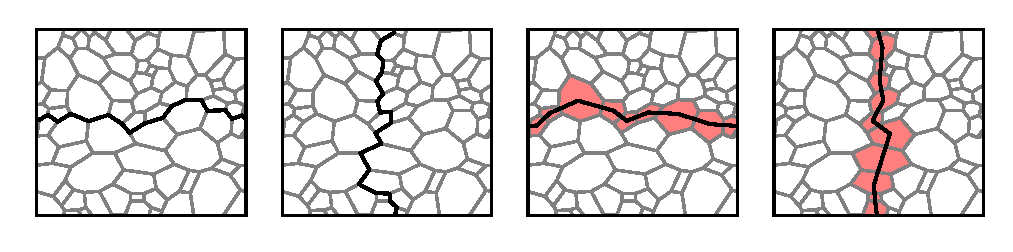
\includegraphics[width=1\textwidth,height=\textheight]{figure_code/amk_chapter/loops_and_dual_loops/loops_and_dual_loops}
\caption[{Topological Loops and Dual Loops}]{(Left) The two topological flux operators of the toroidal lattice. These do not correspond to any face of the lattice, but rather measure flux that threads through the major and minor axes of the torus. This shows a particular choice. Yet, any loop that crosses the boundary is gauge equivalent to one of or the sum of these two loop. (Right) The two ways to transport vortices around the diameters. These amount to creating a vortex pair, transporting one of them around the major or minor diameters of the torus and, then, annihilating them again.}
\label{fig:loops_and_dual_loops}
\end{figure}
}

\begin{lstlisting}[language=Python]
\end{lstlisting}
